\documentclass[aspectratio=169,xcolor=table]{beamer}
%aspcetratio >> 1610 169 149 54 43 32
%The themes:
\usetheme[style=default]{mharvellous}
%\usetheme[style=classic]{mharvellous}
%\usetheme[style=dark]{mharvellous}
%\usetheme[style=mracula]{mharvellous}
%*--------------------------------------------------
%\usepackage{helvet}
%*--------------------------------------------------
\usepackage{bibunits}  
%\setbeamertemplate{bibliography item}{[\theenumiv]}
\setbeamertemplate{bibliography item}{\insertbiblabel}
\defaultbibliography{bibliography}
%\defaultbibliographystyle{IEEEtran}
%\defaultbibliographystyle{amsalpha}
\defaultbibliographystyle{abntex2-alf}
%\bibliography{bibliography}
%\usepackage[backend=biber,style=alphabetic,citestyle=authoryear]{biblatex}
% \addbibresource{bibliography.bib}
%\usepackage{natbib}
\usepackage{bibentry}
%*--------------------------------------------------
\usepackage{lipsum}
\usepackage{epigraph}
\usepackage{graphicx}
\usepackage{multirow}
%\usepackage{enumitem}
\usepackage{array}
\usepackage{subfig}
%\usepackage{multimedia}
\usepackage{media9}
%\usepackage{pdfpc-movie}
\usepackage{circledsteps}
\usepackage{listings}
\usepackage[normalem]{ulem}
%\usepackage{Sweave}
%\usepackage{xkeyval}
%\usepackage{palatino}
%\usepackage{pgfpages}
\usepackage{float}
%*--------------------------------------------------
\usepackage[timeinterval=1]{tdclock}
%\usepackage[font=Times,timeinterval=1, timeduration=200,resetatpages=all]{tdclock}
%\usepackage[font=Times,timeinterval=10, timeduration=2.0, timedeath=0, fillcolorwarningsecond=white!60!yellow,timewarningfirst=50,timewarningsecond=80,resetatpages=2]{tdclock}
%*--------------------------------------------------
\usepackage{url}
\usepackage{tabularx,booktabs}
\usepackage{threeparttable}
\usepackage[absolute, overlay]{textpos}
%*--------------------------------------------------
\usepackage{framed, color}
\usepackage[tikz]{bclogo}
\usepackage{spot}
\setspotlightcolor{red!50}
% %\setspotlightstyle{star, fill=red!50}
% %\setspotlightstyle{star points=7}
\usepackage{color,soul}
%\usepackage{xcolor}
\usepackage{tcolorbox}
\usepackage{xcolor}
\usepackage[export]{adjustbox}
\usepackage{verbatim}
\usetikzlibrary{trees,shapes,arrows}
\usepackage{fancyvrb}
\usepackage{float}
%*--------------------------------------------------
\usepackage{amsmath}
\usepackage{xfrac}
\usepackage{units}
\usepackage{ulem}
%*-------------------------------------------------------------------------------
%\newcolumntype{C}[1]{>{\centering\arraybackslash}m{#1}}
\newcolumntype{L}[1]{>{\raggedright\let\newline\\\arraybackslash\hspace{0pt}}m{#1}}
\newcolumntype{C}[1]{>{\centering\let\newline\\\arraybackslash\hspace{0pt}}m{#1}}
\newcolumntype{R}[1]{>{\raggedleft\let\newline\\\arraybackslash\hspace{0pt}}m{#1}}
%*-------------------------------------------------------------------------------
%\pgfpagesuselayout{2 on 1}[a4paper,border shrink=5mm]
%\setbeamertemplate{note page}[plain]
%\setbeameroption{show notes on second screen=bottom}
%*-------------------------------------------------------------------------------
\setbeameroption{hide notes}
%\setbeameroption{show only notes}
%\setbeameroption{show notes on second screen=right}
\setbeamertemplate{note page}{\pagecolor{yellow!5}\insertnote}
%*-------------------------------------------------------------------------------

%*-------------------------------------------------------------------------------
\title              {Exercício estatística}
\subtitle           {Análise parada dos equipamentos de uma planta}
\author             {Anderson Lima, Juliana Santana, Matheus Anselmo, Matheus Seixas}
\email              {nome@site.com}
\advisor            {Orientador: Marco A. dos Reis}
\institute          {Robótica e Sistemas Autônomos, Senai Cimatec}
\date               {Janeiro de 2022}
% \ulogo        		{Template/logosenaicimatecnegativo}
% \ulogof             {Template/logosenaicimatec2020}
% \ulogoo        		{Template/rosa-logo}
% \ulistelement    	{Template/bullet-white}

%*-------------------------------------------------------------------------------
\graphicspath{{Source/pictures/}}
%*-------------------------------------------------------------------------------
\totalNoSlidesDisabled % To turn off the total number of slides in the footer. Comment this if you want the total number of slides in the footer
%*-------------------------------------------------------------------------------
\begin{document}
%*----------- COVER -------------------------------------------------------------
 \begin{frame}[t,plain]
%*----------- sound--------------------------------
    \includemedia[
        %width=1ex,
        %height=1ex,
        %activate=pageopen, 
        activate=onclick,
        deactivate=onclick,
        %passcontext,
        transparent,
        addresource=./Source/sounds/hip-hop.mp3,
        flashvars={
                    source=./Source/sounds/hip-hop.mp3
                    %&autoPlay=true
                    &autoRewind=true
                    &Play=2s
                    &repeat=always
                    %&Loop=true
        }
    ]
    {}{VPlayer.swf}
%*----------- start-page--------------------------
    \titlepage
    %*----------- notes-------------------------------
    \note[item]{Notes can help you to remember important information. Turn on the notes option.}
\end{frame}
%-
%*----------- SECTIONS ----------------------------------------------------------
%*----------- SLIDE -------------------------------------------------------------
% \begin{frame}[t]{Introdução} 
    
%     \begin{tikzpicture}[thick , scale=1, every  node/.style={scale =0.75}]
%         \node[at=(current  page.center)]
%         {
%             % Created by tikzDevice version 0.12.3.1 on 2022-01-16 03:35:37
% !TEX encoding = UTF-8 Unicode
\begin{tikzpicture}[x=1pt,y=1pt]
\definecolor{fillColor}{RGB}{255,255,255}
\path[use as bounding box,fill=fillColor,fill opacity=0.00] (0,0) rectangle (252.94,252.94);
\begin{scope}
\path[clip] (  0.00,  0.00) rectangle (252.94,252.94);
\definecolor{drawColor}{RGB}{0,0,0}
\definecolor{fillColor}{RGB}{255,0,0}

\path[draw=drawColor,line width= 0.4pt,line join=round,line cap=round,fill=fillColor] ( 55.81, 62.61) rectangle ( 79.43, 93.97);
\definecolor{fillColor}{RGB}{255,77,0}

\path[draw=drawColor,line width= 0.4pt,line join=round,line cap=round,fill=fillColor] ( 84.15, 62.61) rectangle (107.77,203.75);
\definecolor{fillColor}{RGB}{255,153,0}

\path[draw=drawColor,line width= 0.4pt,line join=round,line cap=round,fill=fillColor] (112.49, 62.61) rectangle (136.11, 78.29);
\definecolor{fillColor}{RGB}{255,229,0}

\path[draw=drawColor,line width= 0.4pt,line join=round,line cap=round,fill=fillColor] (140.83, 62.61) rectangle (164.45,188.06);
\definecolor{fillColor}{RGB}{204,255,0}

\path[draw=drawColor,line width= 0.4pt,line join=round,line cap=round,fill=fillColor] (169.17, 62.61) rectangle (192.79, 78.29);
\definecolor{fillColor}{RGB}{128,255,0}

\path[draw=drawColor,line width= 0.4pt,line join=round,line cap=round,fill=fillColor] (197.52, 62.61) rectangle (221.13,125.34);
\end{scope}
\end{tikzpicture}

%         };
%     \end{tikzpicture}

%     \note[item]{Notes can help you to remember important information. Turn on the notes option.}
% \end{frame}

%-
%*----------- SLIDE -------------------------------------------------------------
% \begin{frame}[t]{Introdução}

%     \begin{figure}
%         \subfloat[1° Mês]
%         \centering
%         {
%         \begin{tikzpicture}
%             \begin{tikzpicture}[thick , scale=0.5, every  node/.style={scale =0.5}]
%                 \node[at=(current  page.center)]
%                 {
%                     % Created by tikzDevice version 0.12.3.1 on 2022-01-16 03:35:37
% !TEX encoding = UTF-8 Unicode
\begin{tikzpicture}[x=1pt,y=1pt]
\definecolor{fillColor}{RGB}{255,255,255}
\path[use as bounding box,fill=fillColor,fill opacity=0.00] (0,0) rectangle (252.94,252.94);
\begin{scope}
\path[clip] (  0.00,  0.00) rectangle (252.94,252.94);
\definecolor{drawColor}{RGB}{0,0,0}
\definecolor{fillColor}{RGB}{255,0,0}

\path[draw=drawColor,line width= 0.4pt,line join=round,line cap=round,fill=fillColor] ( 55.81, 62.61) rectangle ( 79.43, 93.97);
\definecolor{fillColor}{RGB}{255,77,0}

\path[draw=drawColor,line width= 0.4pt,line join=round,line cap=round,fill=fillColor] ( 84.15, 62.61) rectangle (107.77,203.75);
\definecolor{fillColor}{RGB}{255,153,0}

\path[draw=drawColor,line width= 0.4pt,line join=round,line cap=round,fill=fillColor] (112.49, 62.61) rectangle (136.11, 78.29);
\definecolor{fillColor}{RGB}{255,229,0}

\path[draw=drawColor,line width= 0.4pt,line join=round,line cap=round,fill=fillColor] (140.83, 62.61) rectangle (164.45,188.06);
\definecolor{fillColor}{RGB}{204,255,0}

\path[draw=drawColor,line width= 0.4pt,line join=round,line cap=round,fill=fillColor] (169.17, 62.61) rectangle (192.79, 78.29);
\definecolor{fillColor}{RGB}{128,255,0}

\path[draw=drawColor,line width= 0.4pt,line join=round,line cap=round,fill=fillColor] (197.52, 62.61) rectangle (221.13,125.34);
\end{scope}
\end{tikzpicture}

%                 };
%             \end{tikzpicture}
%         \end{tikzpicture}
%         }
%         \subfloat[2° Mês]
%         \centering
%         {
%         \begin{tikzpicture}
%             \begin{tikzpicture}[thick , scale=0.5, every  node/.style={scale =0.5}]
%                 \node[at=(current  page.center)]
%                 {
%                     % Created by tikzDevice version 0.12.3.1 on 2022-01-16 03:37:54
% !TEX encoding = UTF-8 Unicode
\begin{tikzpicture}[x=1pt,y=1pt]
\definecolor{fillColor}{RGB}{255,255,255}
\path[use as bounding box,fill=fillColor,fill opacity=0.00] (0,0) rectangle (252.94,252.94);
\begin{scope}
\path[clip] (  0.00,  0.00) rectangle (252.94,252.94);
\definecolor{drawColor}{RGB}{0,0,0}
\definecolor{fillColor}{RGB}{255,0,0}

\path[draw=drawColor,line width= 0.4pt,line join=round,line cap=round,fill=fillColor] ( 55.81, 62.61) rectangle ( 91.75, 93.97);
\definecolor{fillColor}{RGB}{255,77,0}

\path[draw=drawColor,line width= 0.4pt,line join=round,line cap=round,fill=fillColor] ( 98.94, 62.61) rectangle (134.88,203.75);
\definecolor{fillColor}{RGB}{255,153,0}

\path[draw=drawColor,line width= 0.4pt,line join=round,line cap=round,fill=fillColor] (142.07, 62.61) rectangle (178.01,203.75);
\definecolor{fillColor}{RGB}{255,229,0}

\path[draw=drawColor,line width= 0.4pt,line join=round,line cap=round,fill=fillColor] (185.19, 62.61) rectangle (221.13,141.02);
\end{scope}
\end{tikzpicture}

%                 };
%             \end{tikzpicture}
%         \end{tikzpicture}
%         }
%         \subfloat[3° Mês]
%         \centering
%         {
%         \begin{tikzpicture}
%             \begin{tikzpicture}[thick , scale=0.5, every  node/.style={scale =0.5}]
%                 \node[at=(current  page.center)]
%                 {
%                     % Created by tikzDevice version 0.12.3.1 on 2022-01-16 03:37:59
% !TEX encoding = UTF-8 Unicode
\begin{tikzpicture}[x=1pt,y=1pt]
\definecolor{fillColor}{RGB}{255,255,255}
\path[use as bounding box,fill=fillColor,fill opacity=0.00] (0,0) rectangle (252.94,252.94);
\begin{scope}
\path[clip] (  0.00,  0.00) rectangle (252.94,252.94);
\definecolor{drawColor}{RGB}{0,0,0}
\definecolor{fillColor}{RGB}{255,0,0}

\path[draw=drawColor,line width= 0.4pt,line join=round,line cap=round,fill=fillColor] ( 55.81, 62.61) rectangle (104.44, 79.22);
\definecolor{fillColor}{RGB}{255,77,0}

\path[draw=drawColor,line width= 0.4pt,line join=round,line cap=round,fill=fillColor] (114.16, 62.61) rectangle (162.78,203.75);
\definecolor{fillColor}{RGB}{255,153,0}

\path[draw=drawColor,line width= 0.4pt,line join=round,line cap=round,fill=fillColor] (172.51, 62.61) rectangle (221.13,112.42);
\end{scope}
\end{tikzpicture}

%                 };
%             \end{tikzpicture}
%         \end{tikzpicture}
%         }
%         \end{figure}

%     \note[item]{Notes can help you to remember important information. Turn on the notes option.}
% \end{frame}

%*----------- SLIDE -------------------------------------------------------------
% \begin{frame}[c]{Quantidade de paradas}
%     \centering
%     \begin{figure}
%         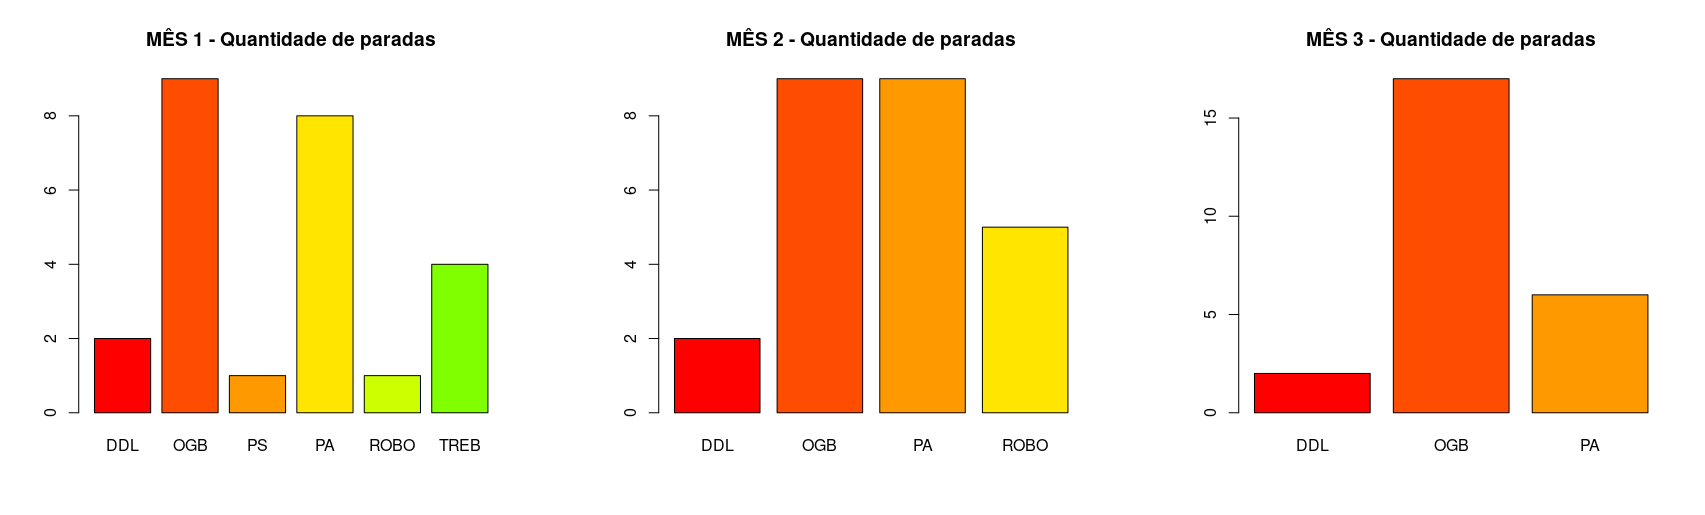
\includegraphics[ width=1\textwidth]{qtdparadas.png}
%         %\caption{.}
%     \end{figure}


%     \note[item]{Notes can help you to remember important information. Turn on the notes option.}
% \end{frame}
%-

%*----------- SLIDE -------------------------------------------------------------
% \begin{frame}[c]{Tempo de parada}
%     \centering
%     \begin{figure}
%         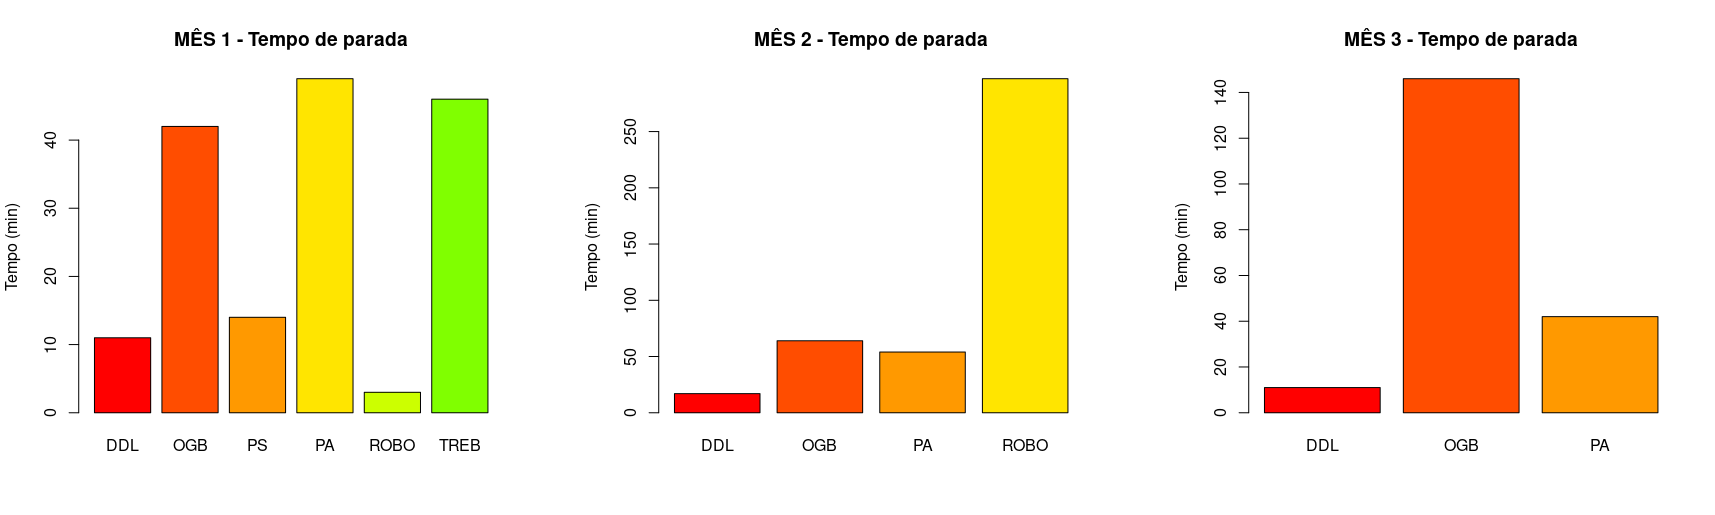
\includegraphics[ width=1\textwidth]{tempoparada.png}
%     \end{figure}

%*----------- notes
%     \note[item]{Notes can help you to remember important information. Turn on the notes option.}
% \end{frame}
%-

%*----------- SLIDE -------------------------------------------------------------
\begin{frame}[c]{Quantidade de paradas}
    \centering
    \begin{figure}
        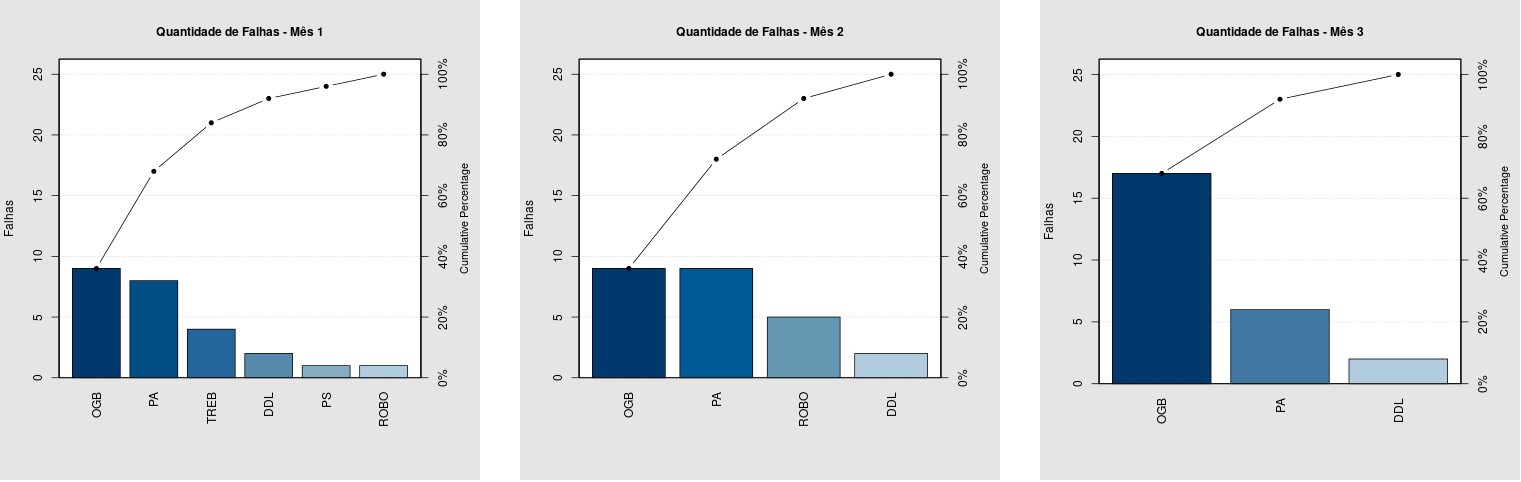
\includegraphics[ width=1\textwidth]{qtd-paradas.png}
        %\caption{.}
    \end{figure}

%*----------- notes
    \note[item]{Notes can help you to remember important information. Turn on the notes option.}
\end{frame}
%-

%*----------- SLIDE -------------------------------------------------------------
\begin{frame}[c]{Tempo de parada}
    \centering
    \begin{figure}
        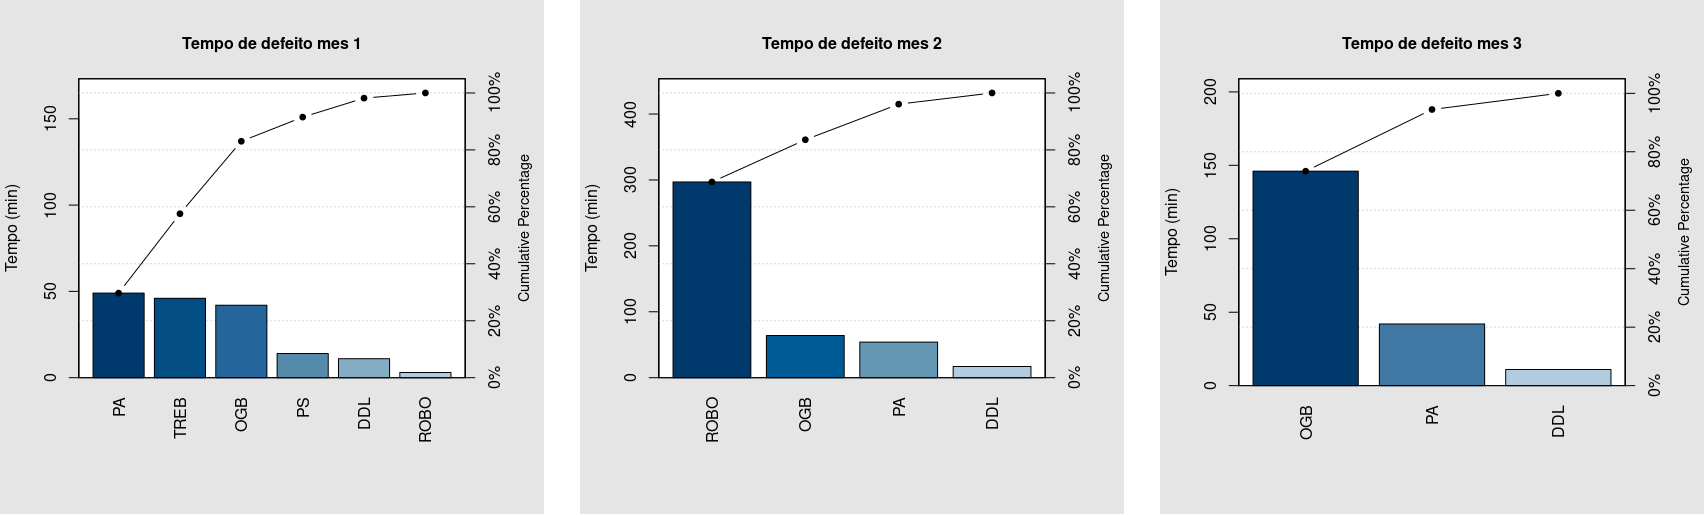
\includegraphics[ width=1\textwidth]{pareto.png}
        %\caption{.}
    \end{figure}

%*----------- notes
    \note[item]{Notes can help you to remember important information. Turn on the notes option.}
\end{frame}
%-
%*----------- SLIDE -------------------------------------------------------------
\begin{frame}[c]{Análise do problema}
    \centering
    \begin{figure}
        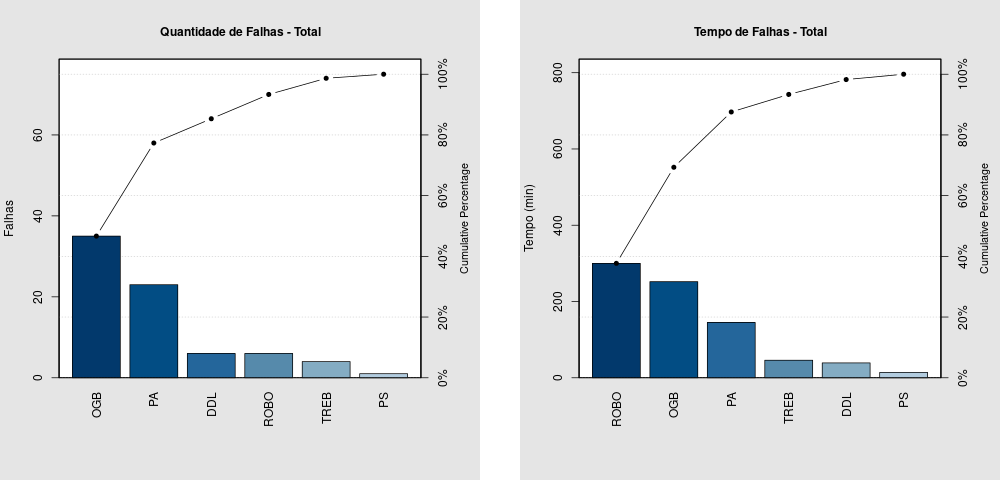
\includegraphics[ width=0.8\textwidth]{tempo-total.png}
        %\caption{.}
    \end{figure}

%*----------- notes
    \note[item]{Notes can help you to remember important information. Turn on the notes option.}
\end{frame}
%-

%*----------- SLIDE -------------------------------------------------------------
\begin{frame}[c]{Análise do problema}
    \begin{table}[ht!]
        \centering
            \caption{Análise considerando a planta}
            \begin{tabular}{|l|c|c|c|} \hline
                \textbf{Dados}&\textbf{Mês 1}&\textbf{Mês 2}&\textbf{Mês 3}\\ \hline
                Quantidade de falhas & 25  & 25  & 25\\ \hline
                Tempo parada &  165 min  & 432 min  &  199 min\\ \hline
                Tempo operacional & 9600 min & 9600 min & 9600 min \\ \hline
                Tempo disponível & 9435 min  & 9168 min  & 9401 min\\ \hline
                MTBF  & 6.29 h  & 6.112 h &  6.267 h\\ \hline
                MTTR  & 6.6 min  & 17.28 min &  7.96 min\\ \hline
            \end{tabular}
        \end{table}
%*----------- notes
    \note[item]{Notes can help you to remember important information. Turn on the notes option.}
\end{frame} 
%-

%*----------- SLIDE -------------------------------------------------------------
\begin{frame}[c]{Análise do problema}
    \centering
        \begin{table}[ht!]
            \centering
                \caption{Análise considerando os equipamentos}
                \begin{tabular}{|l|c|c|c|} \hline
                    \textbf{Dados}&\textbf{\Circled[outer color=mracula7, inner ysep=10pt]{\textcolor{red}{Open Gate - B}}}&\textbf{Pinça Automática}&\textbf{Robô}\\ \hline
                    Quantidade de falhas & \textcolor{red}{35}  & 23  & 6\\ \hline
                    Tempo parada &  252 min  & 145 min  &  300 min\\ \hline
                    MTTR  & 7.2 min  & 6.30 min &  50 min\\ \hline
                \end{tabular}
            \end{table}

%*----------- notes
    \note[item]{Notes can help you to remember important information. Turn on the notes option.}
\end{frame}
%-
% %----------------------------------------------------SLIDE------------------
 \begin{frame}[t, allowframebreaks]{References}
 %\frametitle{References}
%\begin{frame}{Reference}
    %\transboxin[duration=1,direction=30]

    % \begin{bibunit}[plain]
    % \cite{guangyi2018research}.
    % %\cite{kanakia2012}
    % %\cite{agostini2007}
    % %\cite{azuma1997survey}
    % \cite{Buss2005}
  
    % \putbib
    % \end{bibunit}
  
    %\bibliographystyle{IEEEtran}
    %\bibliographystyle{IEEEtranS}
    %\bibliographystyle{IEEEbib}
    \bibliographystyle{abntex2-alf}
    %\bibliographystyle{abntex2-num}
    %\bibliographystyle{abnt-alf}
    \bibliography{bibliography} 
    %\putbib

%*----------- notes
    %\note[item]{Notes can help you to remember important information. Turn on the notes option.}
\end{frame}
%
%-
%*----------- SLIDE-BACKUP ------------------------------------------------------
% \backupbegin
% %
% \begin{frame}{Backup}
%     Test
% %*----------- notes-------------------------------
% \note{Notes can help you to remember important information. Turn on the notes option.}
% \end{frame}
% %-
% \backupend
% %-
%*----------- QUESTIONS ---------------------------------------------------------
\begin{frame}[c,plain]
    \lastpage{
        \begin{center}   
            {\usebeamerfont{title} Questions?}\\[3ex] 
            %\hspace{1.5cm} 
            juliana.maria@fbter.org.br
        \end{center}
    }
    
    %*----------- notes---------------------------------
    \note[item]{Notes can help you to remember important information. Turn on the notes option.}
\end{frame}
%*-------------------------------------------------------------------------------
\end{document}